\documentclass[tikz,border=15pt]{standalone}
\usepackage{tikz}
\usepackage{amsmath}
\usepackage{amssymb}
\usetikzlibrary{shapes.geometric, arrows.meta, positioning, calc, backgrounds, fit, shadows.blur}

\definecolor{navyDark}{HTML}{0B2545}
\definecolor{navyLight}{HTML}{F0F4F8}
\definecolor{navyBorder}{HTML}{134074}

\definecolor{emeraldDark}{HTML}{0E6251}
\definecolor{emeraldLight}{HTML}{E8F8F5}
\definecolor{emeraldBorder}{HTML}{16A085}

\definecolor{purpleDark}{HTML}{512E5F}
\definecolor{purpleLight}{HTML}{F4ECF7}
\definecolor{purpleBorder}{HTML}{8E44AD}

\definecolor{amberDark}{HTML}{7D6608}
\definecolor{amberLight}{HTML}{FEF9E7}
\definecolor{amberBorder}{HTML}{D4AC0D}

\definecolor{crimsonDark}{HTML}{78281F}
\definecolor{crimsonLight}{HTML}{FDF2E9}
\definecolor{crimsonBorder}{HTML}{C0392B}

\definecolor{slateDark}{HTML}{2C3E50}
\definecolor{slateLight}{HTML}{F8F9FA}
\definecolor{slateBorder}{HTML}{BDC3C7}

\begin{document}
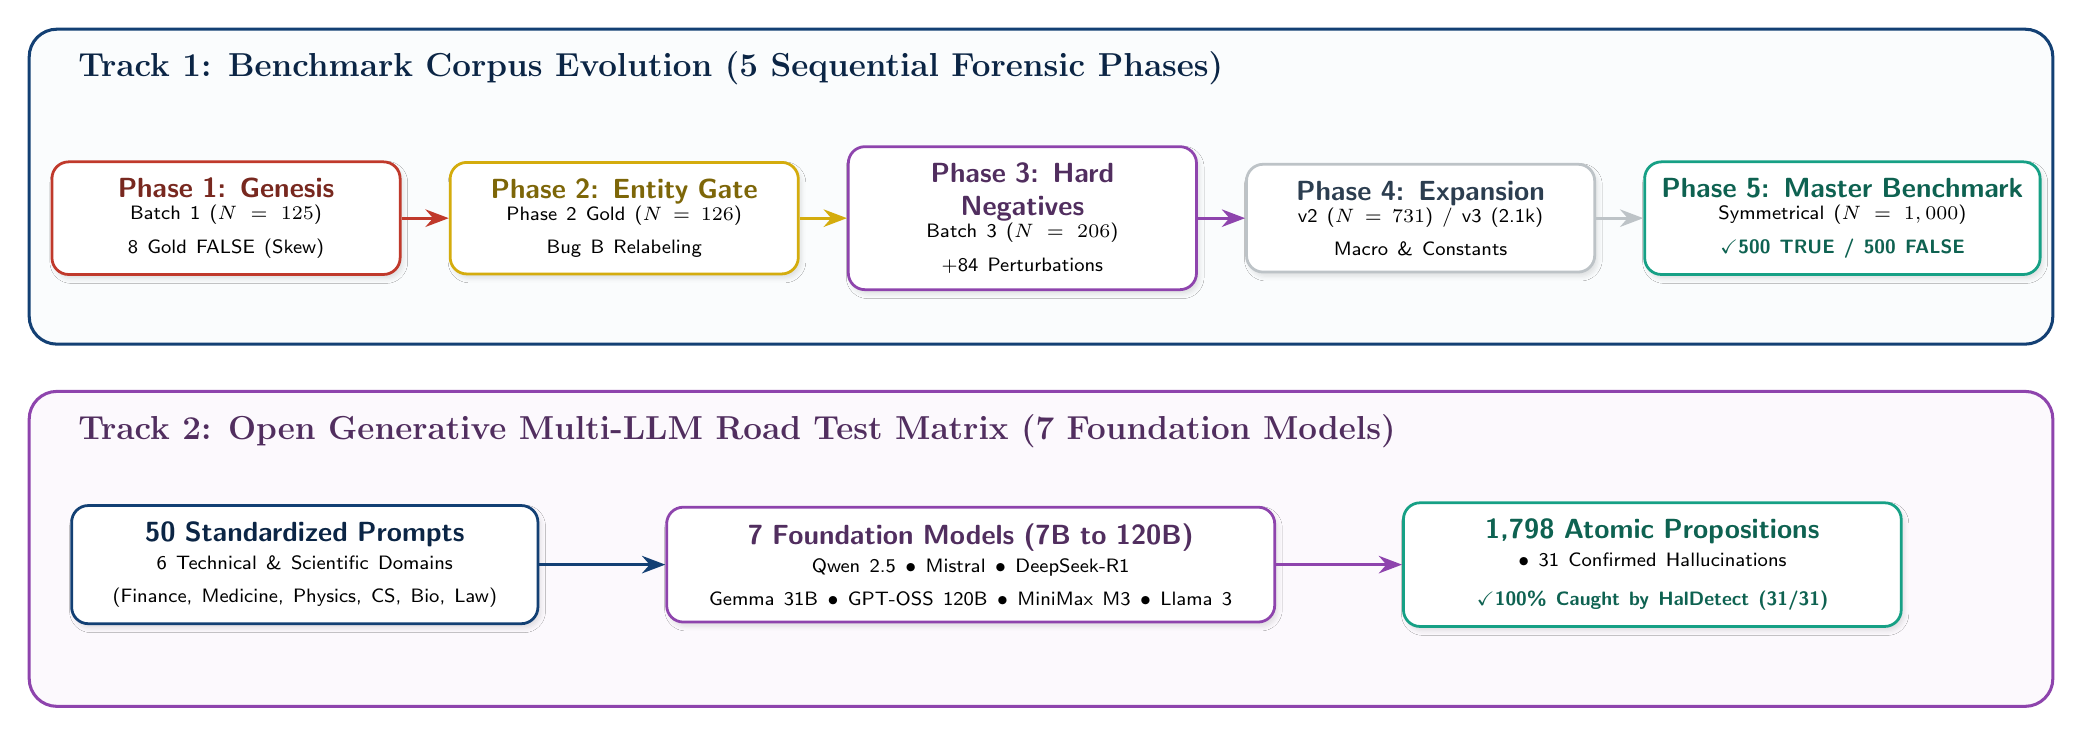
\begin{tikzpicture}[
    font=\sffamily,
    >=Stealth,
    trackbox/.style={
        draw=#1Border, fill=#1Light!30, line width=1.1pt, rounded corners=10pt
    },
    phasebox/.style={
        draw=#1Border, fill=white, line width=1.0pt, rounded corners=6pt,
        blur shadow={shadow blur steps=4, shadow xshift=1pt, shadow yshift=-1.5pt, shadow opacity=12},
        align=center, inner sep=6pt
    },
    wire/.style={
        ->, line width=1.2pt, draw=#1Border
    }
]

% ==================== TRACK 1: BENCHMARK CORPUS EVOLUTION ====================
\draw[trackbox=navy] (-0.5, 0.4) rectangle (25.2, 4.4);
\node[anchor=west, font=\bfseries\large, text=navyDark] at (0.0, 3.9) {Track 1: Benchmark Corpus Evolution (5 Sequential Forensic Phases)};

\node[phasebox=crimson, minimum width=4.2cm, text width=4.0cm] (p1) at (2.0, 2.0) {
    \textbf{\color{crimsonDark} Phase 1: Genesis}\\
    \scriptsize Batch 1 ($N=125$)\\
    \scriptsize 8 Gold FALSE (Skew)
};

\node[phasebox=amber, right=0.6cm of p1, minimum width=4.2cm, text width=4.0cm] (p2) {
    \textbf{\color{amberDark} Phase 2: Entity Gate}\\
    \scriptsize Phase 2 Gold ($N=126$)\\
    \scriptsize Bug B Relabeling
};

\node[phasebox=purple, right=0.6cm of p2, minimum width=4.2cm, text width=4.0cm] (p3) {
    \textbf{\color{purpleDark} Phase 3: Hard Negatives}\\
    \scriptsize Batch 3 ($N=206$)\\
    \scriptsize +84 Perturbations
};

\node[phasebox=slate, right=0.6cm of p3, minimum width=4.2cm, text width=4.0cm] (p4) {
    \textbf{\color{slateDark} Phase 4: Expansion}\\
    \scriptsize v2 ($N=731$) / v3 (2.1k)\\
    \scriptsize Macro \& Constants
};

\node[phasebox=emerald, right=0.6cm of p4, minimum width=4.8cm, text width=4.6cm] (p5) {
    \textbf{\color{emeraldDark} Phase 5: Master Benchmark}\\
    \scriptsize Symmetrical ($N=1,000$)\\
    \scriptsize \textbf{\color{emeraldDark}\checkmark 500 TRUE / 500 FALSE}
};

\draw[wire=crimson] (p1) -- (p2);
\draw[wire=amber] (p2) -- (p3);
\draw[wire=purple] (p3) -- (p4);
\draw[wire=slate] (p4) -- (p5);

% ==================== TRACK 2: MULTI-LLM ROAD TEST ====================
\draw[trackbox=purple] (-0.5, -4.2) rectangle (25.2, -0.2);
\node[anchor=west, font=\bfseries\large, text=purpleDark] at (0.0, -0.7) {Track 2: Open Generative Multi-LLM Road Test Matrix (7 Foundation Models)};

\node[phasebox=navy, minimum width=5.8cm, text width=5.5cm] (t2_prompts) at (3.0, -2.4) {
    \textbf{\color{navyDark} 50 Standardized Prompts}\\
    \vspace{2pt}
    \scriptsize 6 Technical \& Scientific Domains\\
    \scriptsize (Finance, Medicine, Physics, CS, Bio, Law)
};

\node[phasebox=purple, right=1.6cm of t2_prompts, minimum width=7.6cm, text width=7.3cm] (t2_models) {
    \textbf{\color{purpleDark} 7 Foundation Models (7B to 120B)}\\
    \vspace{2pt}
    \scriptsize Qwen 2.5 $\bullet$ Mistral $\bullet$ DeepSeek-R1\\
    \scriptsize Gemma 31B $\bullet$ GPT-OSS 120B $\bullet$ MiniMax M3 $\bullet$ Llama 3
};

\node[phasebox=emerald, right=1.6cm of t2_models, minimum width=6.2cm, text width=5.9cm] (t2_props) {
    \textbf{\color{emeraldDark} 1,798 Atomic Propositions}\\
    \vspace{2pt}
    \scriptsize $\bullet$ 31 Confirmed Hallucinations\\
    \vspace{2pt}
    \scriptsize \textbf{\color{emeraldDark}\checkmark 100\% Caught by HalDetect (31/31)}
};

\draw[wire=navy] (t2_prompts) -- (t2_models);
\draw[wire=purple] (t2_models) -- (t2_props);

\end{tikzpicture}
\end{document}
